\documentclass{article}

% If you're new to LaTeX, here's some short tutorials:
% https://www.overleaf.com/learn/latex/Learn_LaTeX_in_30_minutes
% https://en.wikibooks.org/wiki/LaTeX/Basics

% Formatting
\usepackage[utf8]{inputenc}
\usepackage[margin=1in]{geometry}
\usepackage[titletoc,title]{appendix}

% Math
% https://www.overleaf.com/learn/latex/Mathematical_expressions
% https://en.wikibooks.org/wiki/LaTeX/Mathematics
\usepackage{amsmath,amsfonts,amssymb,mathtools}

% Images
% https://www.overleaf.com/learn/latex/Inserting_Images
% https://en.wikibooks.org/wiki/LaTeX/Floats,_Figures_and_Captions
\usepackage{graphicx,float}

% Tables
% https://www.overleaf.com/learn/latex/Tables
% https://en.wikibooks.org/wiki/LaTeX/Tables


% Algorithms
% https://www.overleaf.com/learn/latex/algorithms
% https://en.wikibooks.org/wiki/LaTeX/Algorithms
\usepackage[ruled, vlined]{algorithm2e}
\usepackage{algorithmic}

% Code syntax highlighting
% https://www.overleaf.com/learn/latex/Code_Highlighting_with_minted
% \usepackage{minted}
%\usemintedstyle{borland}

% References
% https://www.overleaf.com/learn/latex/Bibliography_management_in_LaTeX
% https://en.wikibooks.org/wiki/LaTeX/Bibliography_Management
\usepackage{biblatex}
\addbibresource{references.bib}

\usepackage{hyperref}
\hypersetup{
    colorlinks=true,
    linkcolor=blue,
    filecolor=magenta,      
    urlcolor=cyan,
}

% Title content
\title{AMATH 582 Homework 2: Gabor Transform and Spectrogram for Audio Analysis}
\author{Hongda Li}
\date{\today}

\begin{document}

\maketitle

% Abstract
\begin{abstract}
   In this paper, we are interested in applying the principal of Gabor filtering on real world audio data. Our objective is to utilize different filtering techniques using wavelets to extract out sounds for certain instrument in the audio data. In addition, we also discuss the best way of choosing parameters for Gabor filtering to get the best visualizations for the spectrogram. The results we present are musical notes of the guitar solo and bass solo for 2 rock songs. 
\end{abstract}


\section{Introduction and Overview}
    
    \par\hspace{1.1em}
    The objective is to reproduce the musical scores for a clip taken from the start of the song ``\textit{Sweet Child O' Mine}"  by Guns N' Roses and a guitar solo from \textit``{Comfortably Numb}" by Pink Floyd. We deploy the technique of first using a Shannon Filter on the whole audio to filter out only the frequencies for the instruments that we are interested in, using common knowledge and some basics in music, and then we use Gabor transform to find the best temporal and frequencies resolutions. Finally, we present a way to visualize the spectrogram, and an algorithm to identify the notes with some basics in music theory. In addition, we also explored ways of truncating the audio data so that it runs more efficiently.

\section{Theoretical Background}
    \par\hspace{1.1em}
    The Gabor transform consider the additional usage of a kernel function in the time frequencies, preferably a function that has bounded L2 Norm over the real complex domain. And this is discussed more in details in \cite{kutz_2013_pg324}, we will summarize the important piece here. 
    \begin{equation*}\tag{1}\label{eqn:1}
        g_{\tau, w}(\tau) = \exp(i\omega \tau)g(\tau - t)
    \end{equation*}
    \par
    $\omega$ is the multiplier for the Fourier Kernel. $g$ is a bounded function for filtering signal near $t$. A specific case of the Gabor transform is called the Short Time Fourier Transform(STFT), where we consider a real symmetric matrix to be the kernel. Together with the function $f(\tau)$ representing the signal, we have: 
    \begin{equation*}\tag{2}\label{eqn:2}
        \widetilde{f_g}(t, w) = \int_{-\infty}^{\infty} f(\tau)g(\tau - t)\exp(-i\omega t) d\tau
    \end{equation*}
    \par
    Notice that, the variance under the time and frequencies domain are bounded by some constant. This means that, shortening the width of the kernel will reduce Frequency resolution while increasing the with will reduce time resolution. % Citation here! 
    The problem can be addressed with some oversampling to produce better visualization to compensate. In addition, we consider the usage of several wavelet function for filtering in the time and frequency domain of the signal. 
    \begin{equation*}\tag{wavelet.G}\label{eqn:wavelet.G}
        g(\tau; t, w):=\exp \left(
            -
            \left(
                \frac{\tau - t}{\frac{\sqrt{2}w}{2}}
            \right)^2
        \right)
    \end{equation*}
    \begin{equation*}\tag{wavelet.S}\label{eqn:wavelet.S}
        g(\tau; t, w):=
        \begin{cases}
            1 & |\tau - t| \le w/2 \\ 0 & |\tau - t| > w/2
        \end{cases}
    \end{equation*}
    Where each of the wavelet function (Will be referred to as filter in the text) has one time parameter $\tau$ as the input, and its location and with is controlled by the parameters: $t, w$. In the case of the Gaussian Filter, $w$ means a distribution with $2w$ standard deviation. For computational purposes, the filtering processing using wavelets are implemented as element-wise vector multiplications and the STFT is implemented via FFT with a for loop that slide the kernel through the domain.


\section{Algorithm Implementation and Development}
    \par\hspace{1.1em}
    Two core parts of the algorithm is the parameters for the STFT, the implementations of STFT and the conversion between time domain vector and the frequencies domain vector, other aspects of the algorithm will be discussed as we view the results. The whole procedure of the processing any given audio can be summarized by: 
    \begin{enumerate}
        \item[1.] Setting up the parameters for the spectrogram, choosing a section of the music to analyze.
        \item[2.] FFT on the data, filter out a range of frequencies that the instrument is plying in with the Shannon Filter. 
        \item[3.] Create the spectrogram, truncate it to get the best view for the musical scores, and find out the peaking frequencies. 
    \end{enumerate}
    \subsection{Time to Frequencies Domain Conversion}
        \par\hspace{1.1em}
        The time domain vector is by a vector with the same length as the number of floats in the audio data. As common knowledge, digital audio data usually are sampled $480000$ times second (Uncompressed m4a format). 
        \begin{algorithm}\label{alg:1}
            \begin{algorithmic}[1]
                \STATE{\textbf{Input: }TimeVec}
                \STATE{n := length(TimeVec); L := TimeVec(end) - TimeVec(1);}
                \IF{n is even}
                    \STATE{hz:=$\frac{2\pi}{L}[0: n/2 - 1, -n/2: -1]$}
                \ELSE
                    \STATE{hz:=$\frac{2\pi}{L}[0, 1:(n - 1)/2, -(n - 1)/2:-1]$}
                \ENDIF
                \STATE{hz:= $\frac{\text{hz}}{2\pi}$}
                \STATE{\textbf{Output: } FFTshift(hz)}
            \end{algorithmic}\caption{Converting Time Domain to Frequencies Domain}
        \end{algorithm}
        \par
        Notice that, depending on the parity of the width of the signal, we need to partition the corresponding frequencies domain differently. In the case of even number of partitions, we want $0$ appears at index $n/2-1$ after the fftshift, assuming index start with $0$, and we want $0$ to be at index $\lfloor n/2\rfloor$ after fftshift assuming index starts with $0$. Most importantly, we need to divide it by $2\pi$ to actually obtain the frequencies for the audio.
        
    \subsection{Creation of spectrogram Using STFT}
        \par\hspace{1.1em}
        The next part is the creation of the spectrogram. We implement the width of the filter to be relative to the window's size, and the window's size is simply the total length divides by the number of partitions we want. This is convenient when we sync up the STFT with the bars of music, which helps us get better results and visualization.
        \begin{algorithm}\label{alg:2}
            \begin{algorithmic}[1]
                \STATE{\textbf{Input:} TimeVec: Tvec, Audio: A, RelWidth: W, Number of Partitions: N, WaveletFunction: g}
                \STATE{\textbf{Initialize: }SpectroMatrix}
                \STATE{dt := (Tvec(end) - Tvec(1))/n}
                \STATE{Hz := Input Tvec into \hyperref[alg:1]{Algorithm 1}}
                \FOR{II = 0:N - 1}
                    \STATE{t := Tvec(0) + II*dt}
                    \STATE{F := g(Tvec; Tvec(1) + II*dt + dt/2, W*dt)}
                    \STATE{Signal := F*A}
                    \STATE{Signal := fftshift(fft(Signal))}
                    \STATE{Signal := Filter out excessive frequencies using Hz vector.}
                    \STATE{SpecMatrix(:, II + 1) = Signal}
                    \STATE{SpecMatrix(:, II + 1) = Normalize the II + 1 th row of SpecMatrix, and put it into log scale}
                \ENDFOR
                \STATE{\textbf{Output:} Tvec, Hz, SpecMatrix}
            \end{algorithmic}\caption{Creating spectrogram with STFT}
        \end{algorithm}
        \par
        This algorithm (\hyperref[alg:1]{Algorithm 2}) is generic for all audio and wavelet function: A, and $g$. The variable ``RelWidth:W'' represents the with of the wavelet relative to the with of the partition of the signal in time domain, this adds more flexibility for simple oversampling, in addition, if ``N $\times$ W": is set to be a constant, then the amount of oversampling is kept unchanged
        \par
        In addition, extra processing (line 12 in \hyperref[alg:2]{Algorithm 2}) is involved to make better presentation on the spectrogram, trimming of frequencies that is negative and outside the range of the instrument we are interested in, and present it on a lot scale to scale down the relative sizes of the frequencies constant making the spectrogram more invisible. 
    \subsection{Global Frequencies Filtering and Audio Truncations}
        \par\hspace{1.1em}
        By common knowledge, music are written in bars of notes in Chromatic Scale or the Diatonic Scales for pop songs (Diatonic Scale is in the Chromatic Scale). Each note in Chromatic Scale increments by a multiplier of $2^{1/12}$ in term of frequencies (A semi-tone). An instrument such as guitar usually operates inside a range of 3 octaves (12 Semi-tone per octave). 
        \par
        The reasoning of filtering out the frequencies for just the instrument makes us easier to identify particular instruments using the spectrogram. Implementations wise this is achieved via applying a Shannon Filter to the FFT of an audio section we are interested in, and then Inverse Transform it back. The process acts as a band pass filter and it isolate one of the instruments from other instruments. 
        \par
        Audio is truncated either by seconds, or by BPM (Beats per minute), both are implemented. The reasoning is that, music repeats around a theme with some variations, and they are located in sections of bars. Truncating the music in terms of bars reduce loads for computations, it also makes better visualization for the spectrogram. 

\section{Computational Results}
    \subsection{GNR: Notes and Spectrogram}
        \par\hspace{1.1em}
        For the clip from GNR (\textit{Sweet Child O' Mine}), a shannon filter located at the interval $[220, 800]$ is applied, it covers the alto an tenor range of the music, the expected range for the guitar.
        There are 8 bars of music in total, each 2 bars repeats and builds on the same motif, the first 3 sections build on variations, while the 4th one repeats the first 2 bars. 
        \par
        After running the routine highted in the previous section, the result is shown in \hyperref[fig:1]{figure 1}. The melody is written on the C\# major key. The music score is: C\#3,C\#4, G\#3, F\#3,F\#4, G\#3, F4, G\#3, the 2 bars is then repeated with variations on the first, second and 4th keys.   
        \par
        Computationally, The first bars of music is partitioned into 128 sections, and the Gabor kernel is the Gaussian function with a relative width of 4, this allows the audio to be super-sampled, allowing for an smoother image. Other wavelets for STFT is experimented however Gaussian and Shannon filter was proven to produce the best spectrogram and the most accurate results. 

        \begin{figure}[h]\label{fig:1}
            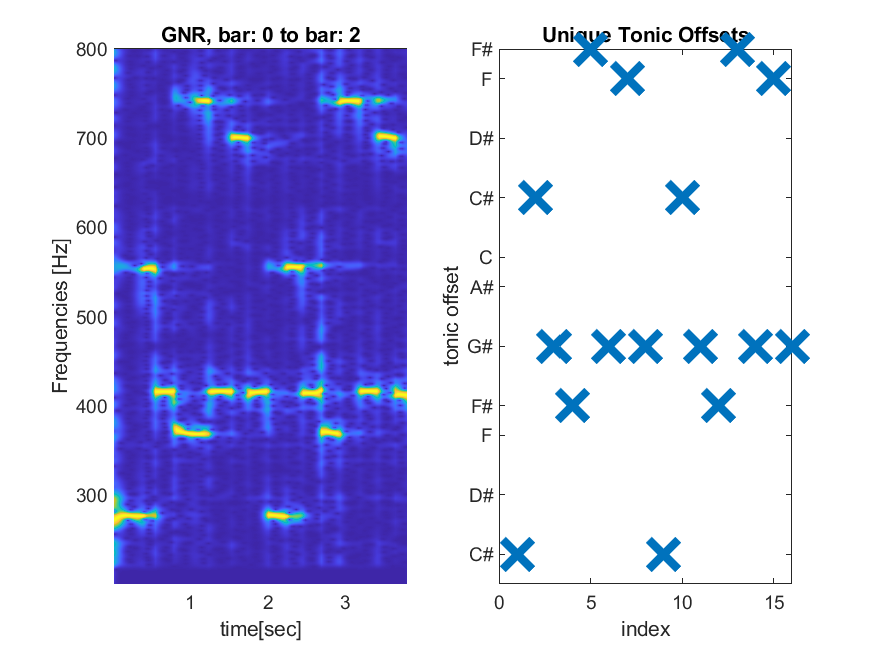
\includegraphics[width=12cm]{gnr-spectro.png}
            \centering
            \caption{GNR: Spectrogram of the Guitar, Gaussian Wavelet}
        \end{figure}
    \subsection{Floyd: Bass Notes and Spectrogram}
        \par\hspace{1.1em}
        The bass of the song ``\textit{Comfortably Numb}'' performs a Basso Obstinate on the G minor scale. A Shannon Filter is used globally to filter out frequencies in the $[50, 110]$ hertz Because that is the expected acoustic range off the instrument. The result is presented in \hyperref[fig:2]{Figure 2}. It shows one bars of the score that is played byt the bass which is repeated through out the audio clip. The music score is: 
        D1, B1, A1, G1, F1, D1. However, it's unclear whether the key B, and D are presented at the same time to create a harmony. 
        \par
        For this example, both the Gaussian and the Shannon Wavelet function is deployed. Take note that \hyperref[fig:2]{Figure 2 Left} shows the spectrogram when the Guassian Wavelet is used and \hyperref[fig:2]{Figure 2 Right} shows the spectrogram when Shannon Wavelet is used. Both Clearly identifies the same frequencies content, however it visually Shannon Wavelet produces sharper image. 
        \par
        The audio clip is partitioned into 64 sections. (Observe how much bigger it is compare to audio clip); and a relative with of 4 is chosen. The choice is justified by the fact that lower acoustic signal need longer window to identify. 
        \begin{figure}[h]
            
            \includegraphics*[width=8cm]{floyd-bass-spectro.png}
            \includegraphics*[width=8cm]{floyd-bass-spectro-shannon.png}
            \caption{Floyd's Bass, Gaussian and Shannon Wavelet}
            \label{fig:2}
        \end{figure}
        
    \subsection{Floyd: Guitar Solo and Spectrogram}
        \par\hspace{1.1em}
        In this section, we will present the spectrogram for the guitar solo in the audio clip. However, due to the virtuosity of the guitar soloist, the music score cannot be presented. More sophisticated algorithm is need to identify complex harmony and melodic contour, unfortunate it's not as simple as STFT. 
        \par
        The routine is run on the whole music clip for Floyd's ``Comfortably Numb'' on the acoustic range of the guitar via global filtering, and the results in shown in: \hyperref[fig:3]{Figure 3}. Please observe the complexity of the melodic contour, and how simple the previous 2 examples are. In this case, multiple notes seems to be played at the same time. The notes are Legato instead of staccato, creating significant challenge for reading the notes from the spectrogram. Simply trick by pulling out the frequencies with the maximal magnitude is not feasible anymore. 

        \begin{figure}[h]
        \centering
            \includegraphics*[width=0.7\linewidth]{floyd-all-guitar.png}    
            \caption{Floyd whole Song Guitar with Shannon Wavelet}
            \label{fig:3}
        \end{figure}

\section{Summary and Conclusions}
    \par\hspace{1.1em}
    The algorithmic frameworks for the STFT can be easily implemented in high level scientific programming language. The visualization process is however, where mostly the works comes in. To get the best out of the digital signal, we need domain specific knowledge for analysis, trial errors to figure out the best window with and discretization of the signal. However, it also shows us that, when dealing with more complex melodic contour and musical articulations, significant challenge is placed on the process of interpreting the spectrogram as music score.
% References
\printbibliography
    
% Appendices
\begin{appendices}

\section{MATLAB Functions}
    
\end{appendices}

\end{document}
